This section is devoted to provide a detailed description of the included video \footnote{Alternatively, the video can be consulted in this link \url{https://www.youtube.com/watch?v=ElxK_95n4lE&feature=youtu.be}}.
%
Especifically, to have a better insight of the benefits provides by our proposal, a simulation with the WFG5 problem is recored.
%
The WFG5 problem is selected given its properties being perhaps under standart parameterization on of the most difficult in the WFG toolkit~\cite{Joel:WFG}.
%
The main peculiarity of this problem dwell in its desceptiveness, which involves several local optimal regions that mislead the search process of the algorithms.
%
Principally, the Pareto geometry of this problem is convex, and such Pareto optimal solutions of the distance parameters have the following values:
%
\begin{equation}\label{ref:Solution}
   x_{i=k+1:n} = 2i \times 0.35
\end{equation}
In addition, in this simulation is taken into account the standard parameterization indicated in the main document, as well the specified configuration.
%
Each algorithm was run with two objectives and two decision variables, whose number of position and distance parameters were set to one, and the number of generations was set to $1000$.
%
The diversity explicitly promoted in the decision variable space by our proposal is until the $50\%$ of the total generations.
%
Since that the R2-EMOA is a steady-state algorithm, each generation is reported as an equivalent to the number of function evaluations.
%

The video is vertically split in two sides, i.e. the left-side and right-side and each one represents the objective space and the decision variable space respectively.
%
In the decision variable space (right-side) each local optimal region is remarked by a horizontal blue line, and the global optimal region is remarked with a horizontal red line.
%
In this configuration, the position and distance parameters are denoted by $x_1$ and $x_2$ respectively, thus according to Equation~\ref{ref:Solution} the Pareto optimal solutions are conformed by the  $x_2=1.4$.
%
The video shows that after ten generations the state-of-the-art-MOEAs have converged prematurely to the deceptive regions, contrarely to the VSD-MOEA which is still exploring.
%
Approximatelly until the $30\%$ of total generations, VSD-MOEA has located three individuals in the global optimal region, and in few generations later ($40\%$) has converged moderately to the optimal region.
%
Thereafter, at the $50\%$ of total generations, VSD-MOEA has converged to the optimal and desired region (red horizontal line) avoiding the remaining sub-optimals (blue horizontal lines).
%
Finally, the remaining generations VSD-MOEA keeps improving the quality of the solutions in the objective space.
%%Figures ONE TWO THREE, are taken of the video and belong to the 0\%, 50\% and 100\% of total generations.
%%
%%\begin{figure}[t]
%%\centering
%%\begin{tabular}{l}
%% 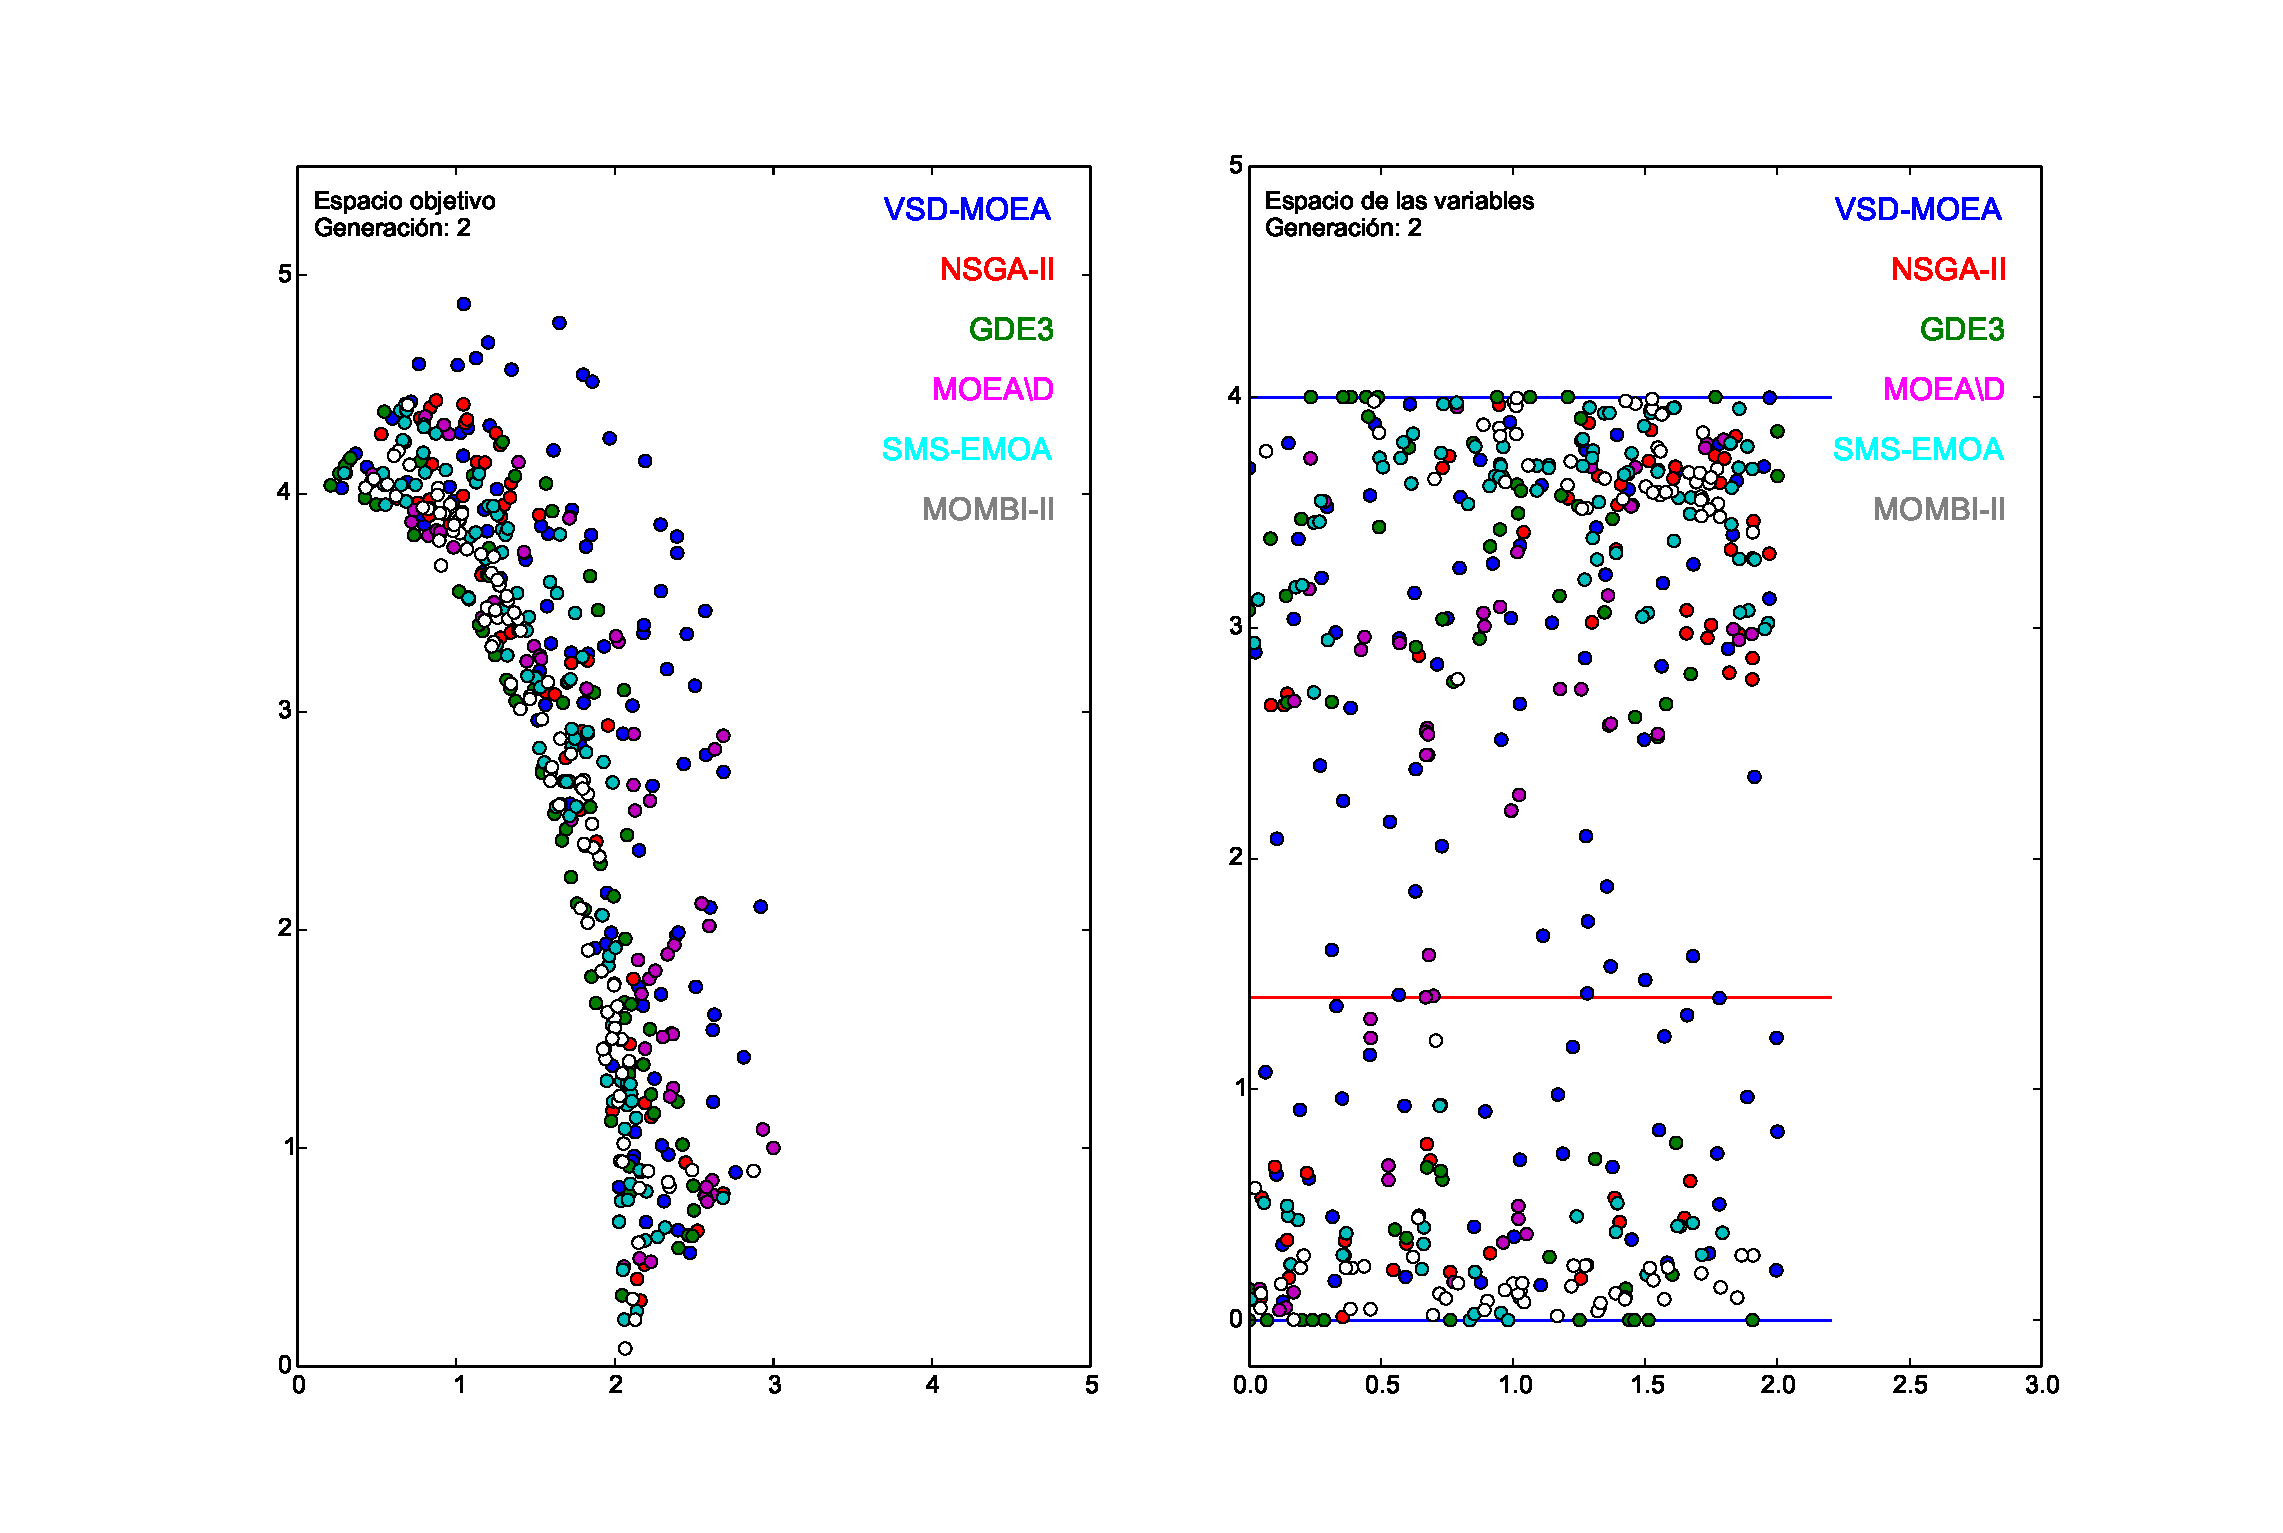
\includegraphics[scale=0.3]{Images/Simulacion_Algoritmo_1.eps}\\[0cm]%[-0.14cm] 
%% 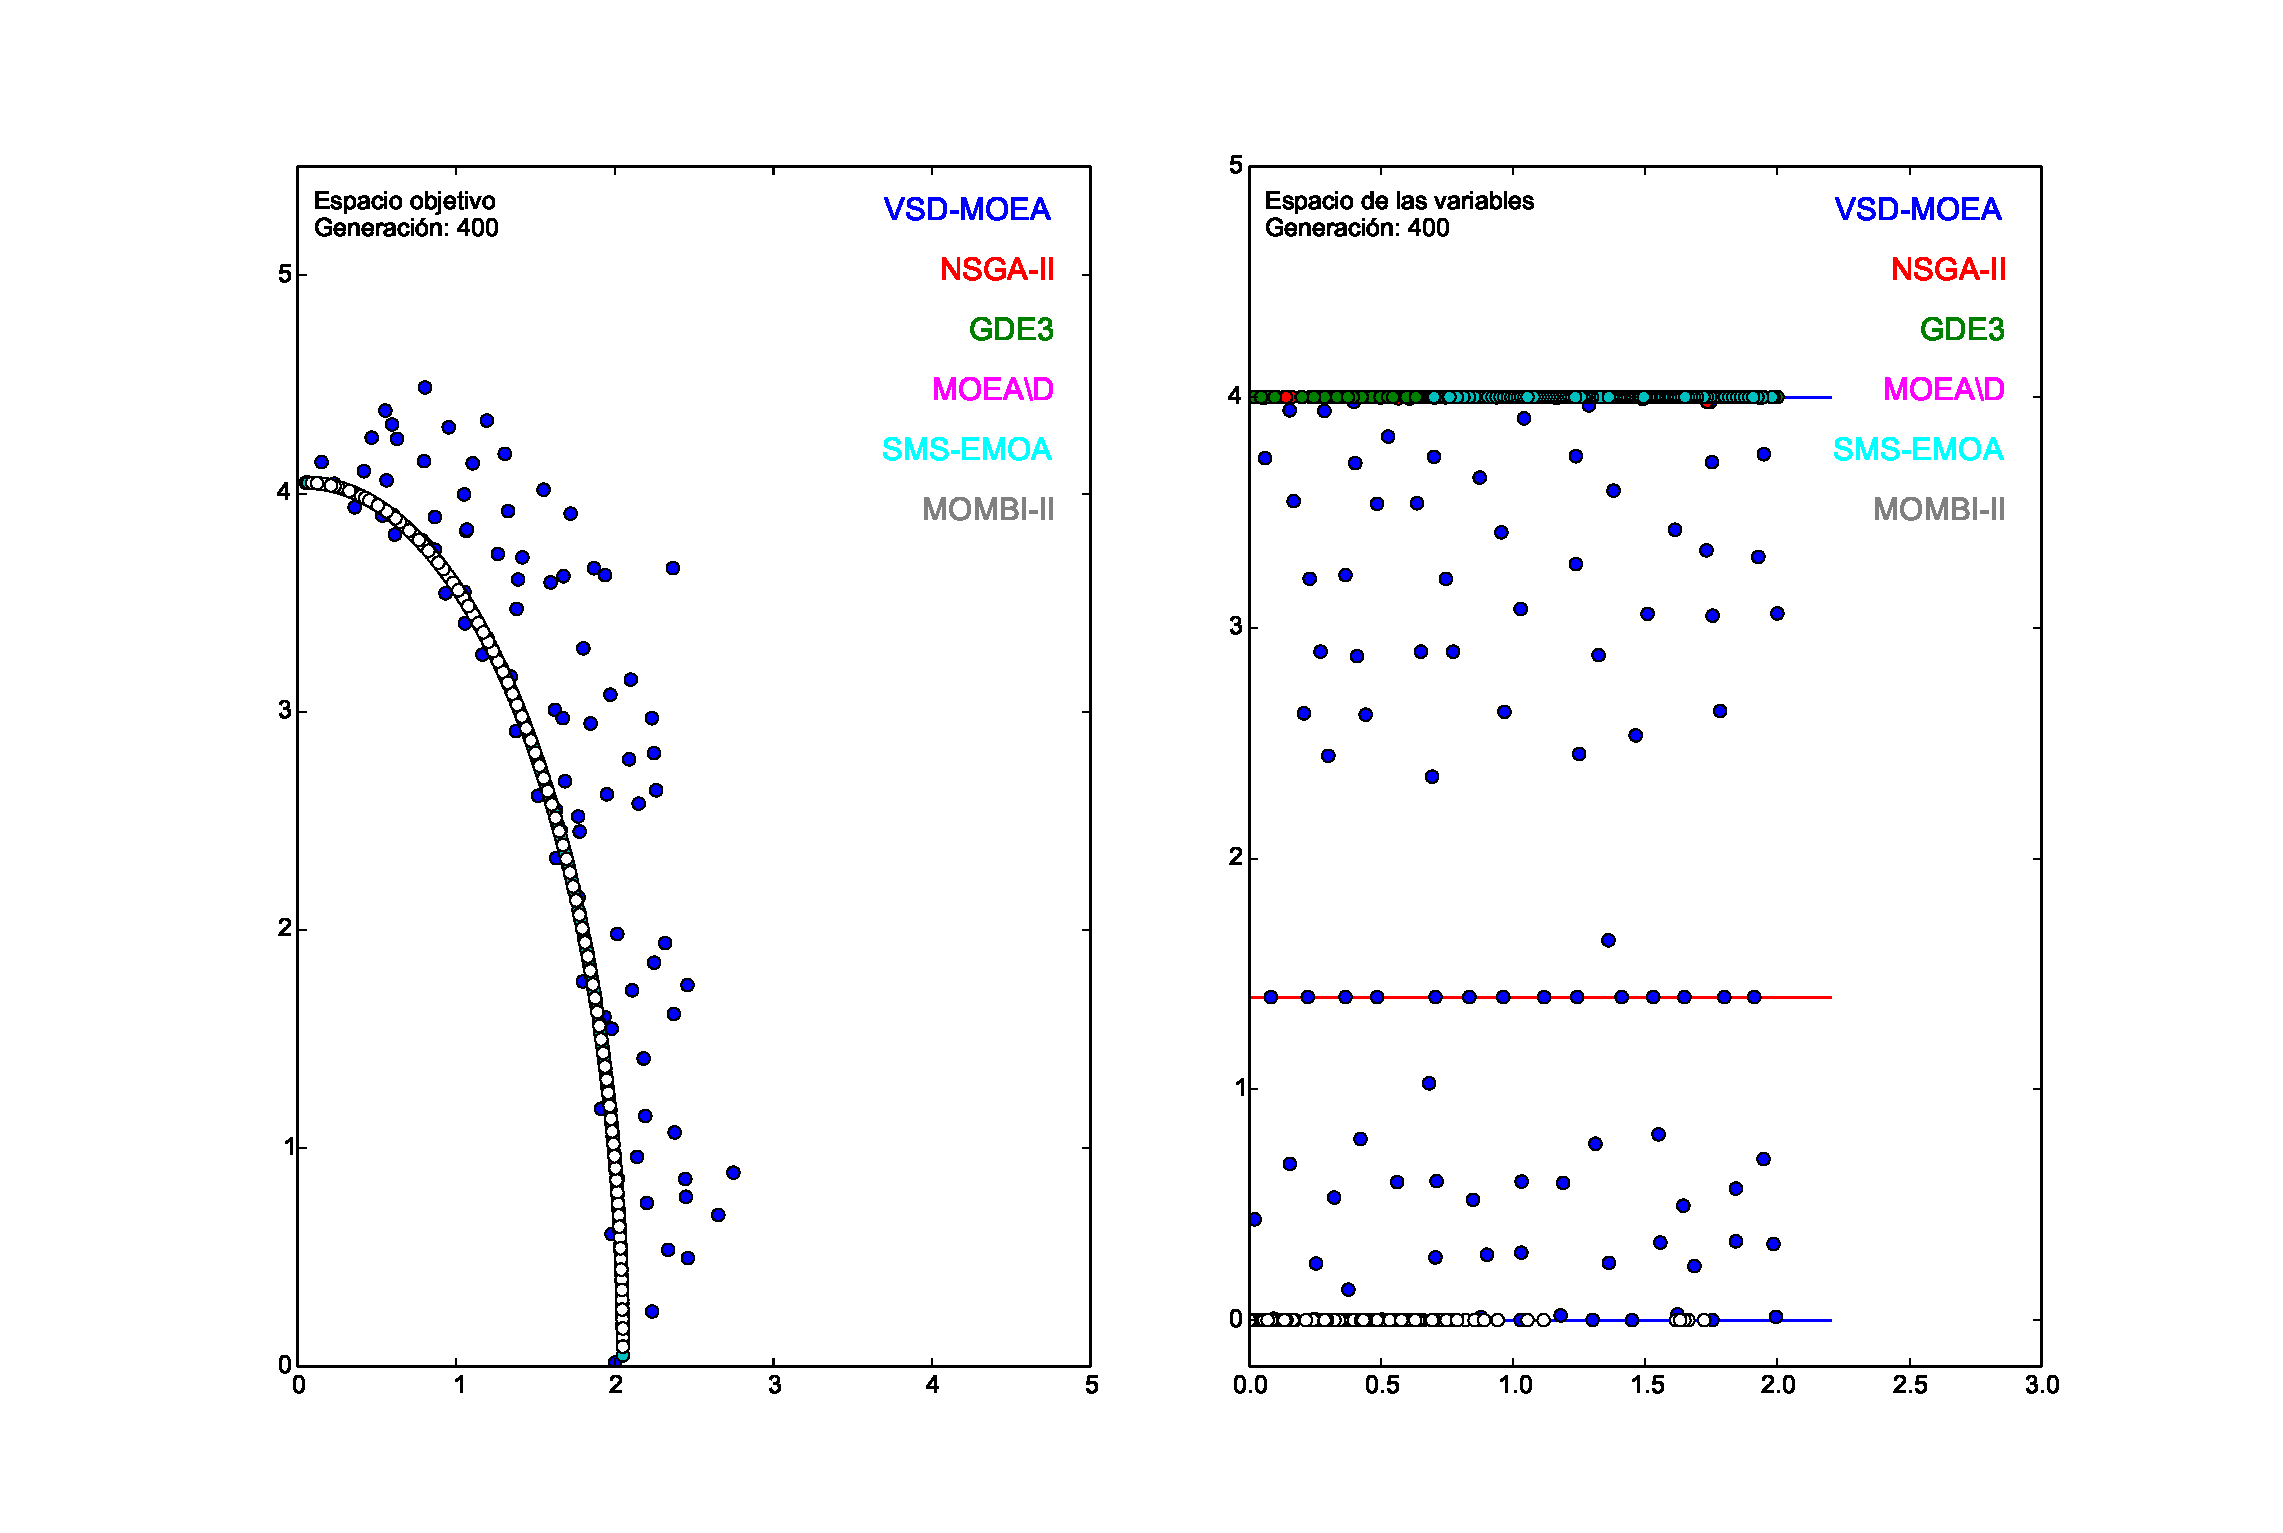
\includegraphics[scale=0.3]{Images/Simulacion_Algoritmo_4.eps}\\[0cm]%[-0.14cm] 
%% 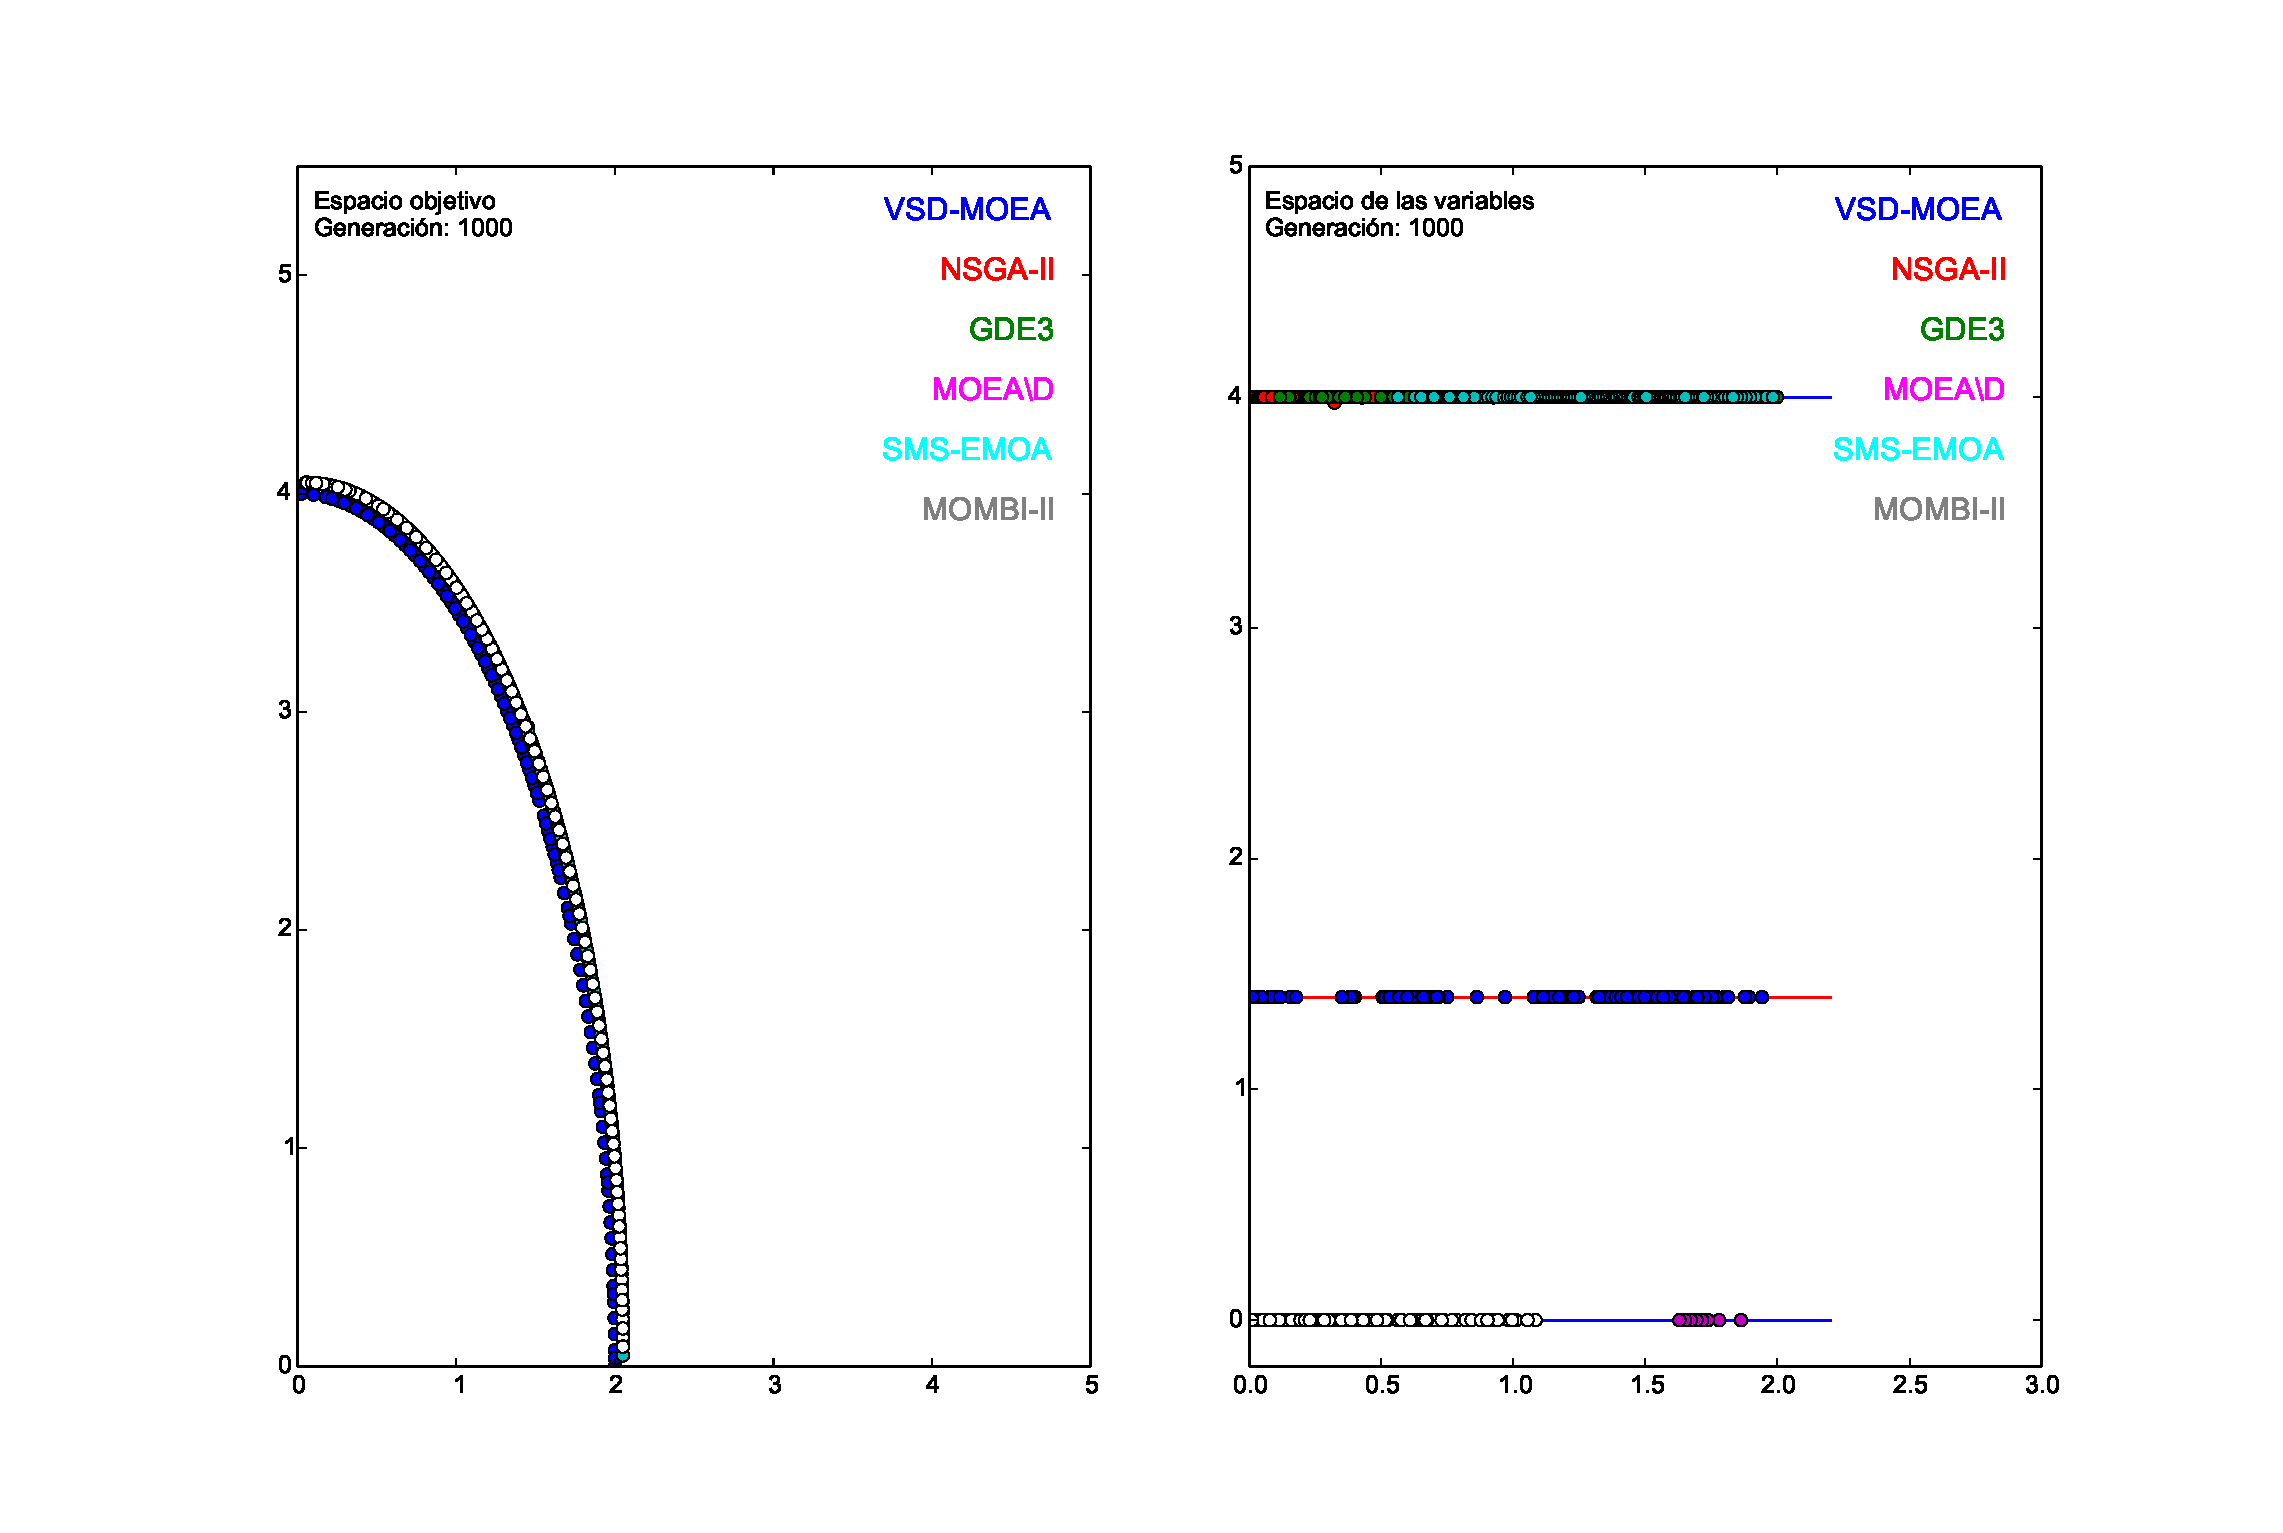
\includegraphics[scale=0.3]{Images/Simulacion_Algoritmo_5.eps}\\[0cm]%[-0.14cm] 
%%\end{tabular}
%%\caption{Performance of \MOEAS{} for the problems with three objectives considering three ranges of stopping criterion: short-term (first row), middle-term (second row) and long-term (third row).}\label{fig:Performance_time_3obj}
%%\end{figure}
